%-------------------------------------------------------------------------------
% 请勿删除本注释
% Free Response Question 3
%
% 指引:
% 如在小问之前有通用问题描述,请放置于此
%-------------------------------------------------------------------------------
\begin{figure}[H]
\centering
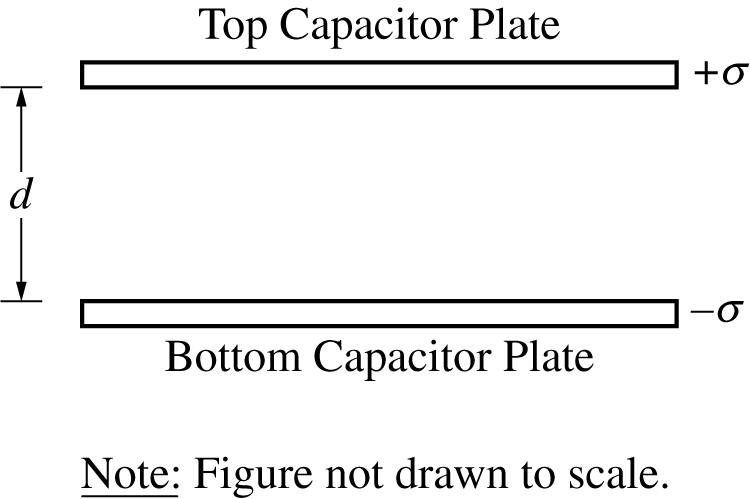
\includegraphics[scale=0.3]{images/img-026-041.png}
\end{figure}

\question
A parallel plate capacitor is connected to a battery, fully charged, and then isolated from the battery. The plates are given equal and opposite charge densities $\sigma$, and the separation between the plates is $d$, as shown in the figure above. The area of each plate has a value of $A$. % 请删除并替换本行,与上一行 \question 之间不要留空行

\begin{parts}

%-------------------------------------------------------------------------------
% 请勿删除本注释
% Part (a)
%
% 指引:
% 如在小问之前有通用问题描述,请放置于此
%-------------------------------------------------------------------------------

\part
Derive an expression for the energy stored in the capacitor. Express your answer in terms of $\sigma, d, A$, and physical constants, as appropriate. % 请删除并替换本行,与上一行 \part 之间不要留空行

%-------------------------------------------------------------------------------
% 请勿删除本注释
% Part (b)
%
% 指引:
% 如在小问之前有通用问题描述,请放置于此
%-------------------------------------------------------------------------------

\begin{figure}[H]
\centering
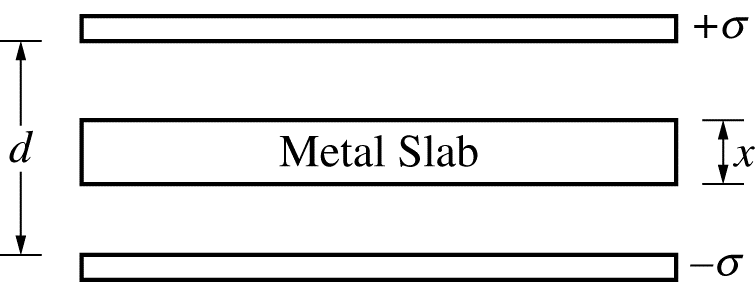
\includegraphics[scale=0.3]{images/img-026-042.png}
\end{figure}

While the capacitor is isolated from the battery, an uncharged metal slab of thickness $x$ and area Ais inserted between the capacitor plates so that it is an equal distance from the two plates, as shown in the figure above.

\part
On the figure above, draw an arrow to indicate the direction of the electric field in the following three regions of space between the capacitor plates. If the electric field is zero in any region, indicate this by writing "E=0" in that region. % 请删除并替换本行,与上一行 \part 之间不要留空行
\begin{subparts}
\subpart The region between the top plate and the metal slab
\subpart The region inside the metal slab
\subpart The region between the metal slab and the bottom plate
\end{subparts}

%-------------------------------------------------------------------------------
% 请勿删除本注释
% Part (c)
%
% 指引:
% 如在小问之前有通用问题描述,请放置于此
%-------------------------------------------------------------------------------

\part
On the lines below, rank the regions according to the magnitude of the electric field, with 1 being the largest magnitude. If any regions have the same magnitude of electric field, give them the same ranking. % 请删除并替换本行,与上一行 \part 之间不要留空行

\underline{\qquad} The region between the top plate and the metal slab

\underline{\qquad} The region inside the metal slab

\underline{\qquad} The region between the metal slab and the bottom plate

%-------------------------------------------------------------------------------
% 请勿删除本注释
% Part (d)
%
% 指引:
% 如在小问之前有通用问题描述,请放置于此
%-------------------------------------------------------------------------------

\part
Is the capacitance of the capacitor with the metal slab greater than, less than, or equal to the capacitance of the original capacitor without the slab? % 请删除并替换本行,与上一行 \part 之间不要留空行

\underline{\qquad}Greater than \qquad \underline{\qquad}Less than \qquad \underline{\qquad}Equal to

Justify your answer.

%-------------------------------------------------------------------------------
% 请勿删除本注释
% Part (e)
%
% 指引:
% 如在小问之前有通用问题描述,请放置于此
%-------------------------------------------------------------------------------

\part
When charged to the original charge density, is the energy stored in the capacitor with the metal slab greater than, less than, or equal to the original energy stored in the capacitor calculated in part (a)? % 请删除并替换本行,与上一行 \part 之间不要留空行

\underline{\qquad}Greater than \qquad \underline{\qquad}Less than \qquad \underline{\qquad}Equal to

Justify your answer.

%-------------------------------------------------------------------------------
% 请勿删除本注释
% Part (f)
%
% 指引:
% 如在小问之前有通用问题描述,请放置于此
%-------------------------------------------------------------------------------
Some physics students conduct an experiment in which they charge the capacitor to the same potential difference, isolate it from the battery, insert the metal slab, and measure the new potential difference across the capacitor. This experiment is repeated with slabs of different thickness. The plot of the potential difference $\Delta V$ across the capacitor as a function of the thickness $x$ of the slab is shown below. A best-fit line for the data has been drawn.

\begin{figure}[H]
\centering
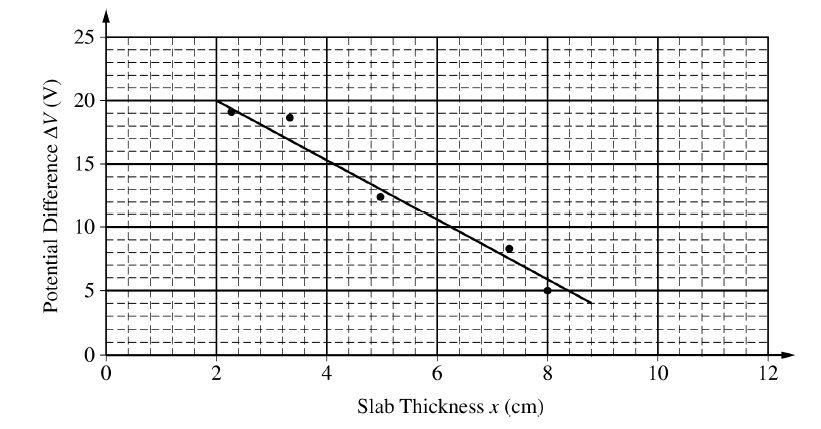
\includegraphics[scale=0.5]{images/3-f.png}
\end{figure}

\part
Use the best-fit line to calculate the following: % 请删除并替换本行,与上一行 \part 之间不要留空行
\begin{subparts}
\subpart $\sigma$, the charge density on the plates
\subpart $d$, the distance between the capacitor plates
\end{subparts}

\end{parts}
